%
% teil2.tex -- Beispiel-File für teil2 
%
% (c) 2020 Prof Dr Andreas Müller, Hochschule Rapperswil
%
% !TEX root = ../../buch.tex
% !TEX encoding = UTF-8
%
%https://blogs.mathworks.com/cleve/2013/10/14/complex-step-differentiation/

\section{Complex-Step-Differentiation}
\label{step:section:complex}
\kopfrechts{Complex-Step-Differentiation}

Neben der automatischen Differentiation mit dualen Zahlen existiert eine weitere numerische Methode zur präzisen Bestimmung von Ableitungen: die \emph{Complex-Step-Differen\-tia\-tion} \cite{step:martins2003}.  
\index{Complex-Step-Differentiation}%
Diese Methode kombiniert die Vorteile numerischer Verfahren mit einer deutlich höheren Genauigkeit als die klassische Finite-Differenzen-Methode.

Ausgangspunkt ist die Erweiterung reeller Funktionen auf den komplexen Zahlenraum \cite{step:squire1998,step:martins2003}. Sei dazu $f:\mathbb{R} \to \mathbb{R}$ eine holomorphe Funktion, die sich analytisch auf $\mathbb{C}$ fortsetzen lässt.  
Wird nun das Argument der Funktion um einen rein imaginären Anteil erweitert, ergibt sich
\begin{equation*}
	f(x + i h),
\end{equation*}
wobei $i$ die imaginäre Einheit mit $i^2 = -1$ ist und $h \in \mathbb{R}$ wiederum eine kleine Schrittweite darstellt.

\subsection{Herleitung der Methode}

Nimmt man die Taylor-Entwicklung (\ref{step:taylor2}) und evaluiert diese am komplexwertigen Punkt $x + ih$ ergibt sich
\begin{equation*}
	f(x + i h) = f(x) + i h f'(x) - \frac{h^2}{2} f''(x) - i \frac{h^3}{6} f^{(3)}(x) + \frac{h^4}{24} f^{(4)}(x) + \dots .
\end{equation*}
Betrachtet man nun den Imaginärteil dieses Ausdrucks, so ergibt sich
\begin{equation*}
	\Im(f(x + i h)) = h f'(x) - \frac{h^3}{6} f^{(3)}(x) + \dots .
\end{equation*}
Unter der Annahme, dass $h$ klein ist, kann die Reihe nach dem ersten Glied abgeschnitten werden, was zu dem Ausdruck
\begin{equation}
	f'(x) \approx \frac{\Im(f(x + i h))}{h}
	\label{step:complexstep}
\end{equation}
für die Ableitung erster Ordnung führt \cite{step:squire1998}.
Im Gegensatz zur Finite-Differenzen-Methode (\ref{step:finitdiff}) tritt hier kein Subtraktionsterm der Form $f(x+h) - f(x)$ auf.  %\label{step:finitdiff}
So wird verhindert, dass bei sehr kleinen Schrittweiten Auslöschung auftritt, die sonst zu erheblichen Rundungsfehlern führen kann.

\subsection{Complex-Step und Cauchy-Riemann-Differentialgleichungen}
Man kann die Complex-Step-Methode auch als Folge der
Cauchy-Riemann-Differential\-gleichungen verstehen.
\index{Cauchy-Riemann-Differentialgleichungen}%
Dazu schreiben wir eine holomorphe Funktion $f(z)$ wieder wie in
Kapitel~\ref{chapter:holomorph} mit Realteil $u(z)$ und Imaginärteil
$v(z)$ als $f(z) = f(x+iy) = u(x,y) + i v(x,y)$.
Die Ableitung $f'(z)$ kann durch partielle Ableitung nach $x$ aus
\begin{equation}
f'(z)
=
\frac{\partial u}{\partial x} + i\frac{\partial v}{\partial x}
\label{step:fpartial}
\end{equation}
erhalten werden.
Für eine Funktion, die auf reellen Argumenten reelle Funktionswerte
annimmt, ist $v(x,0) = 0$ für $x\in \mathbb{R}$.
Daher verschwindet auch die partielle Ableitung von $v$ nach $x$.
Für die Berechnung von $f'(x)$ fällt somit der zweite Term in
\eqref{step:fpartial}
weg.
Die Ableitung wird für reelle Argumente daher
\begin{align}
f'(x)
&=
\frac{\partial u}{\partial x}.
\notag
\intertext{Nach den Cauchy-Riemann-Differentialgleichungen
\eqref{buch:holomorph:holomorph:eqn:cr}
ist dies gleichbedeutend mit}
f'(x)
&=
\frac{\partial v}{\partial y}.
\notag
\intertext{Die partielle Ableitung nach $y$ kann als finite Differenz}
f'(x)
&\approx
\frac{v(x,h) - v(x,0)}{h}
=
\frac{v(x,h)}{h}
=
\frac{\operatorname{Im}f(x+ih)}{h}
\label{step:vpartial}
\end{align}
approximiert werden, wobei wir wiederum $v(x,0)=0$ verwendet haben.
Es ist also erneut die Approximation \eqref{step:complexstep} gefunden
worden.

\subsection{Erfolgsfaktoren}
Zwei Voraussetzungen sind für den Erfolg der Methode verantwortlich:
\begin{enumerate}
\item
Die Berechnung der Ableitung nach dem Realteil $x$ ist auch durch
Berechnung einer Ableitung nach dem Imaginärteil $y$ möglich.
Nur bei holomorphen Funktionen lässt sich aus der einen Ableitung auf
die andere schliessen.
\item
Die Auslöschung verursachende Differenzbildung fällt weg, wenn der
Subtrahend bekanntermassen verschwindet.
In \eqref{step:vpartial} war dies die Eigenschaft, dass $v(x,0)=0$
für reelle $x$ ist.
Die Funktion $f(z)$ muss also für reelle Argumente reelle Werte haben.
\end{enumerate}
Die Methode funktioniert also zur Ableitung von reellen Funktionen, die
eine analytische Erweiterung auf eine Umgebung der reellen Achse 
haben.
In Abschnitt~\ref{buch:analytisch:potenzreihen:nichtanalytisch} wurde
mit einem Beispiel gezeigt, dass nicht jede reelle Funktion eine solche
analytisch Fortsetzung hat.

\subsection{Anwendung der Complex-Step-Methode}

Im Folgenden wird die Methode an zwei Funktionen getestet, einer Polynomfunktion sowie einer analytischen Funktion. 
In beiden Fällen wird gezeigt, dass die Methode in der Lage ist, die erste Ableitung nahezu fehlerfrei zu approximieren.
\begin{beispiel}
Gegeben sei das Polynom $f(x) = x^3 + x^2 + x + 1$, wobei dieses nun durch die Substitution $x \rightarrow x + ih$ erweitert wird. 
Es ergibt sich:
\begin{align*}
	f(x + ih) &= (x + ih)^3 + (x + ih)^2 + (x + ih) + 1 \\
	&= \big(x^3 + 3x^2ih + 3x(ih)^2 + (ih)^3\big) + \big(x^2 + 2xih + (ih)^2\big) + x + ih + 1 \\
	&= x^3 + 3x^2 ih + 3x(i^2 h^2) + i^3 h^3 + x^2 + 2x ih + i^2 h^2 + x + ih + 1 \\
	&= x^3 + 3x^2 ih - 3x h^2 - i h^3 + x^2 + 2x ih - h^2 + x + ih + 1 \\
	&= \big(x^3 + x^2 + x + 1 - 3x h^2 - h^2\big) + i\big(3x^2 h + 2x h + h - h^3\big).
\end{align*}
Zur Approximation der Ableitung wird der Imaginärteil betrachtet:
\begin{align*}
	f'(x) \approx \frac{\Im(f(x + i h))}{h}
	&= 3x^2 + 2x + 1 - h^2.
\end{align*}
Der auftretende Fehlerterm ist somit proportional zu $h^2$, weshalb die Complex-Step-Me\-tho\-de einen Fehler der Ordnung $O(h^2)$ aufweist.
Dies stellt einen wesentlichen Unterschied zur Finite-Differenzen-Methode dar, bei der nach dem Abbruch der Taylor-Entwicklung ein Fehler erster Ordnung $O(h)$ verbleibt.
Bei der Complex-Step-Methode verschwinden hingegen die geraden Potenzen von $ih$ beim Betrachten des Imaginärteils, sodass nach der Division durch $h$ der führende Fehlerterm von quadratischer Ordnung ist.

Für ein hinreichend kleines $h$ kann der Fehlerterm $h^2$ vernachlässigt werden, sodass sich für die Ableitung Lösung
\begin{equation*}
	f'(x) \approx 3x^2 + 2x + 1
\end{equation*}
ergibt.
Damit zeigt sich, dass die Complex-Step-Methode die exakte Ableitung ohne Subtraktionsfehler liefert.
Wie in Abbildung~\ref{fig:complex_step_fehler1} zu erkennen ist, liefert die Complex-Step-Me\-tho\-de im Vergleich zur Finite-Differenzen-Methode eine deutlich höhere Genauigkeit.
\begin{figure} %todo
	\centering
	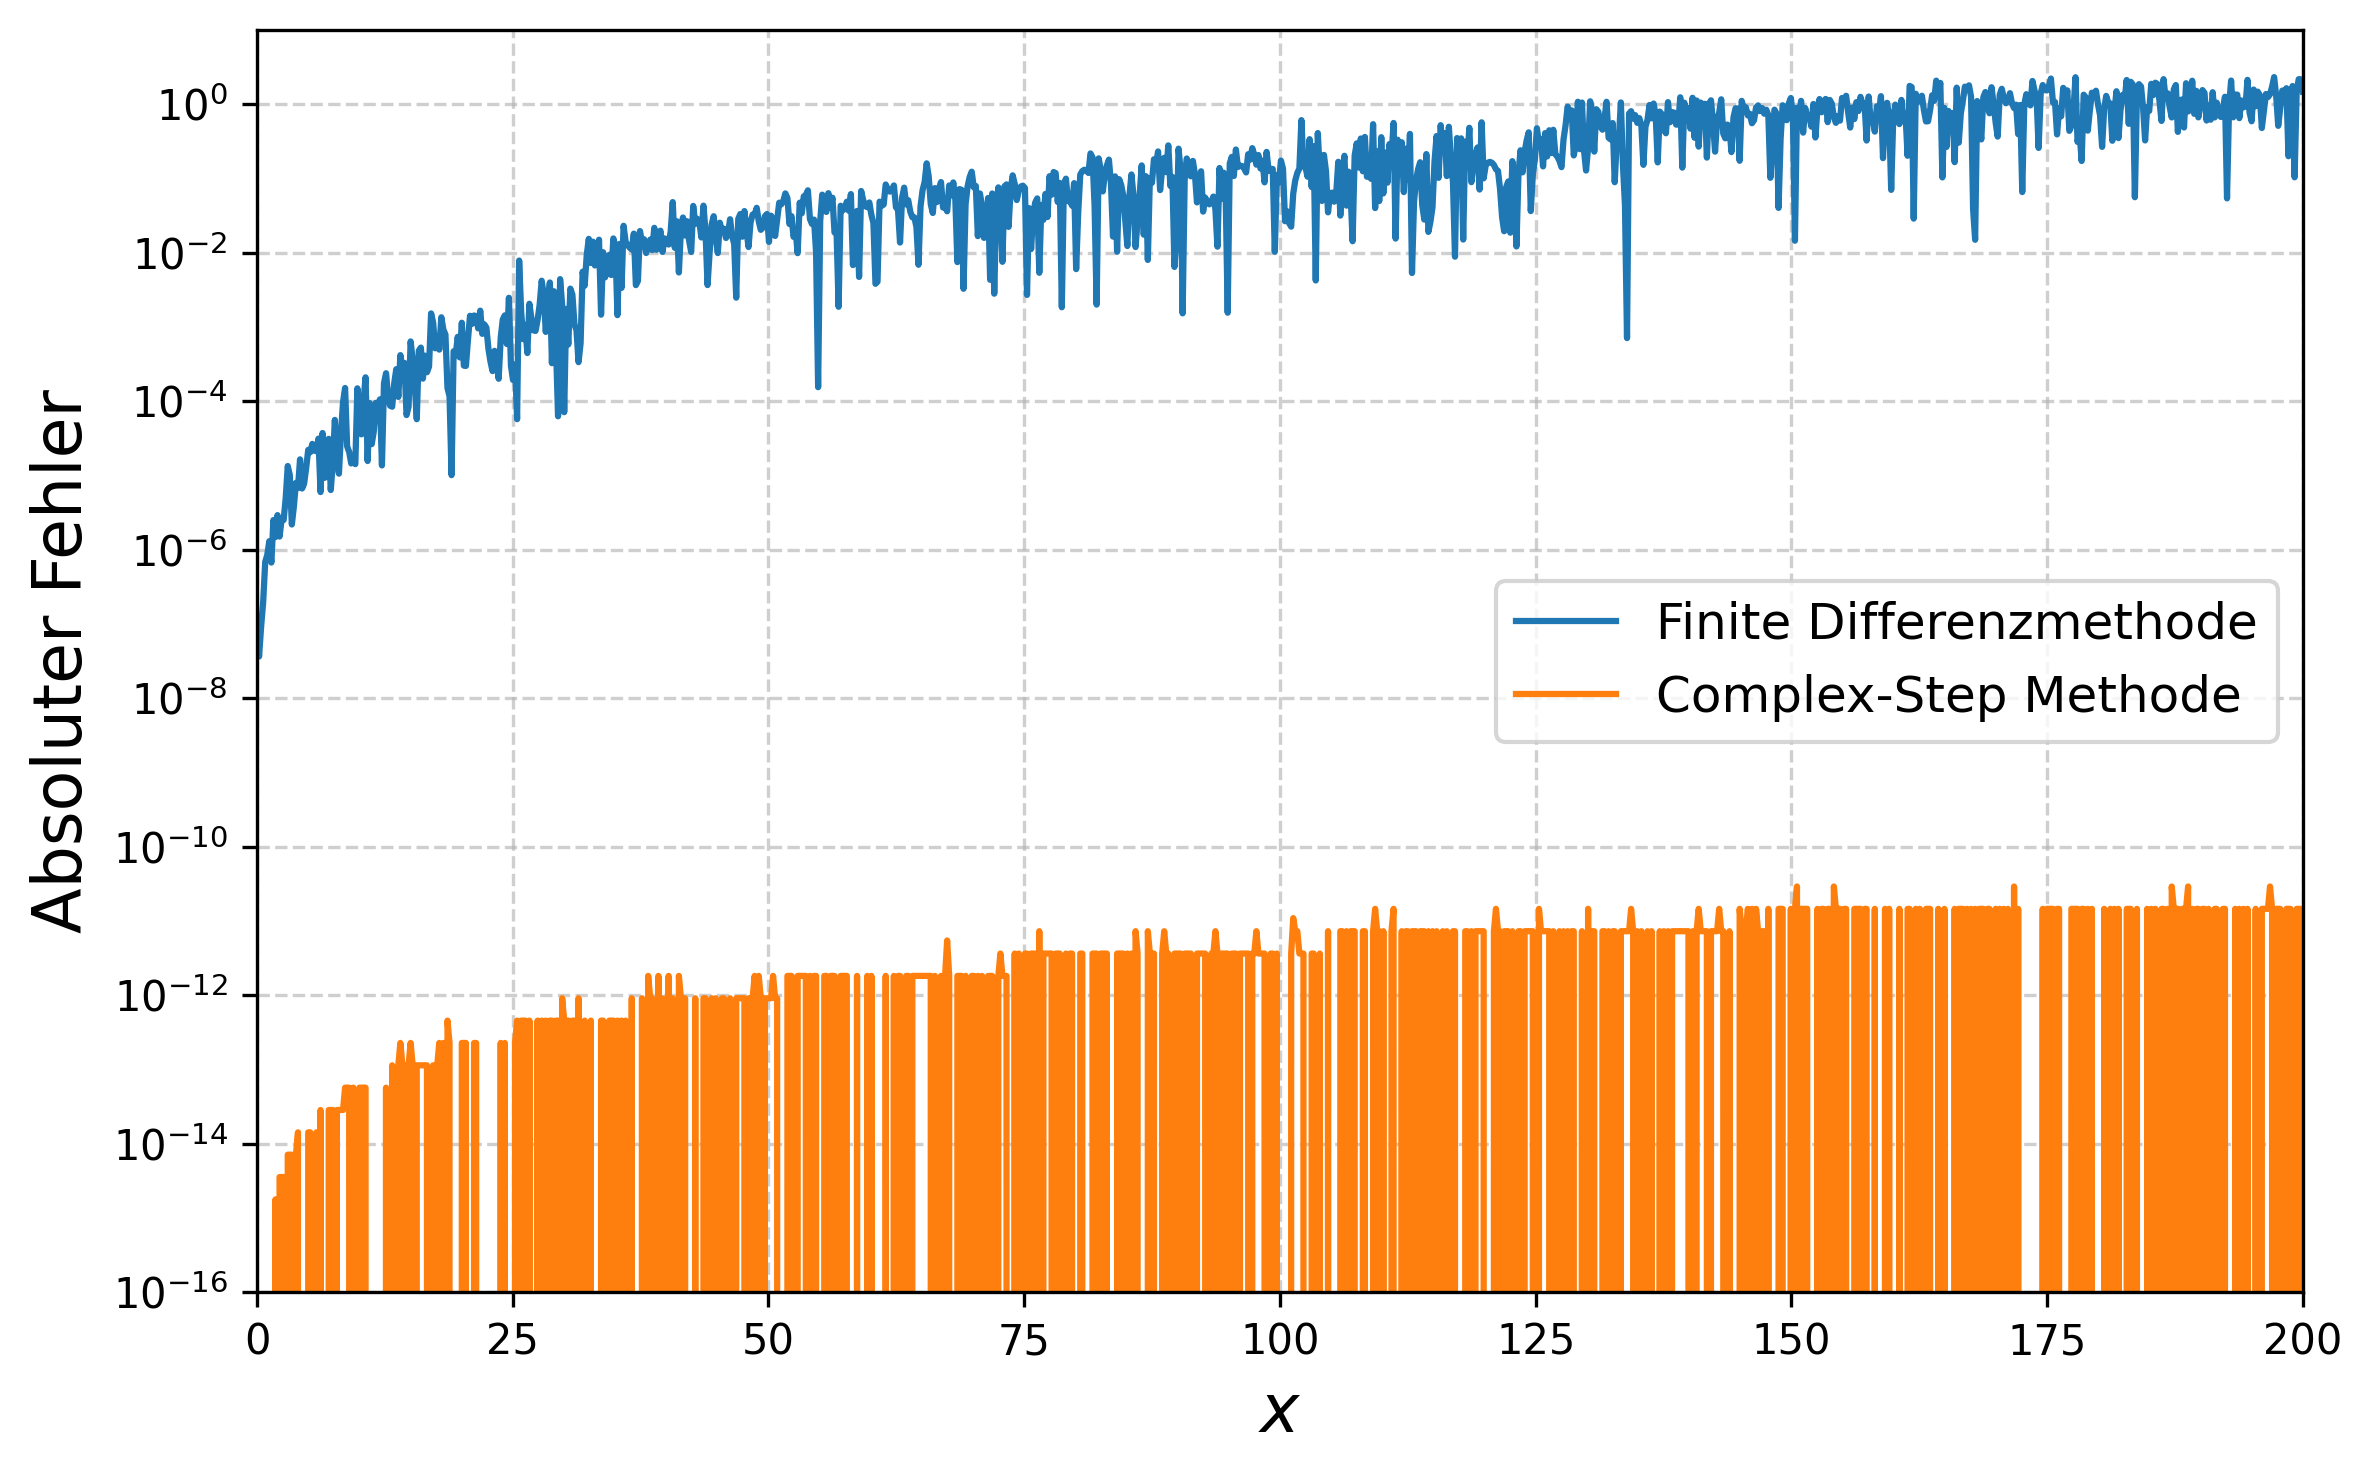
\includegraphics[width=0.8\textwidth]{papers/step/img/complex_step_vergleich1.png}
	\caption{Absoluter Fehler der Ableitung von $f(x) = x^3 + x^2 + x + 1$ 
		für Finite-Differenzen- und Complex-Step-Methode mit einer Schrittweite $h=10^{-9}$.}
	\label{fig:complex_step_fehler1}
\end{figure}
\end{beispiel}
\begin{beispiel}
Gegeben sei die analytische Funktion $f(x) = \sin(x)$. Mittels Erweiterung in die komplexe Ebene $x + ih$ ergibt sich
\begin{align*}
	f(x + ih) &= \sin(x + ih) \\
	&= \sin(x)\cos(ih) + \cos(x)\sin(ih).
\end{align*}
Mithilfe der Kleinwinkelnäherungen $\cos(ih) \approx 1$ und $\sin(ih) \approx ih$ für kleine $h$ lässt sich obiger Ausdruck vereinfachen zu
\begin{equation*}
	f(x + ih) = \sin(x) + ih\cos(x).
\end{equation*}
Zur Approximation der Ableitung wird der Imaginärteil
\begin{align*}
f'(x) \approx \frac{\Im(f(x + i h))}{h}
	&=\cos(x)
\end{align*}
betrachtet.
Somit ergibt sich auch für diese Funktion eine präzise Bestimmung der Ableitung ohne numerisch bedingte Subtraktionsfehler, was durch die in Abbildung~\ref{fig:complex_step_fehler2} dargestellten Ergebnisse bestätigt wird.
\begin{figure} %todo
	\centering
	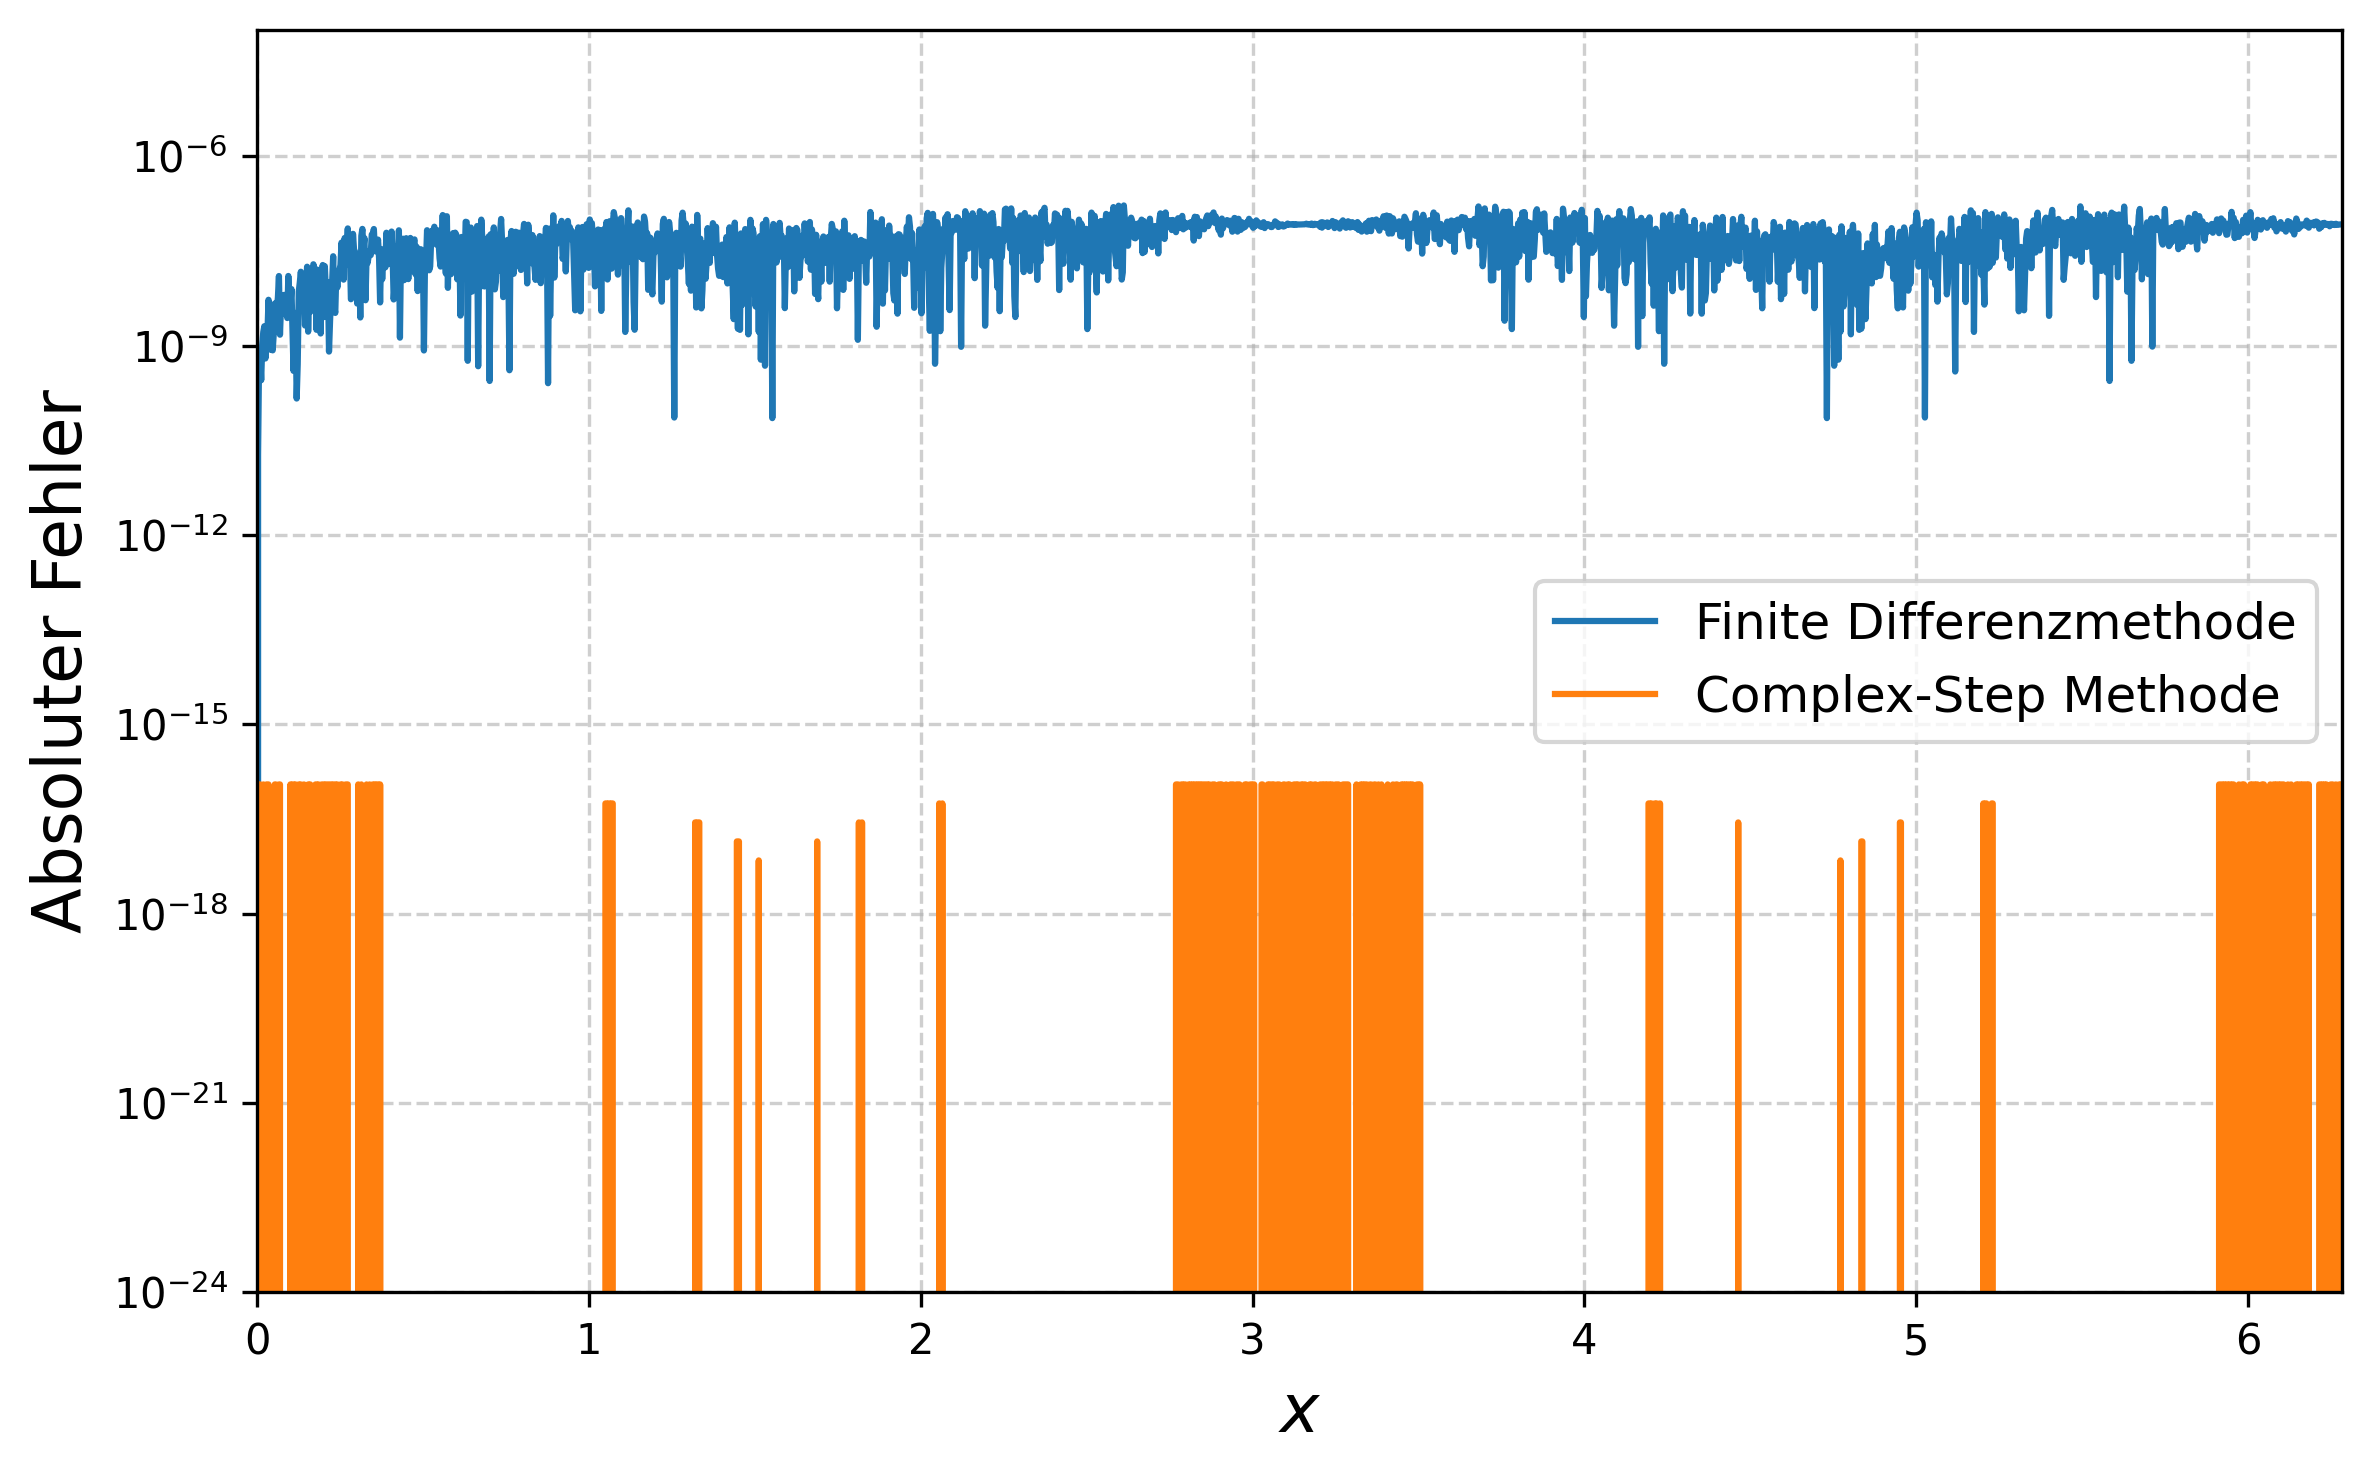
\includegraphics[width=0.8\textwidth]{papers/step/img/complex_step_vergleich2.png}
	\caption{Absoluter Fehler der Ableitung von $f(x) = \sin(x)$ 
		für Finite-Differenzen- und Complex-Step-Methode mit einer Schrittweite $h=10^{-9}$.}
	\label{fig:complex_step_fehler2}
\end{figure}
\end{beispiel}
\subsection{Implementierung in Python}

Die Methode lässt sich in Python äusserst einfach implementieren, da komplexe Zahlen nativ unterstützt werden:
\index{Python}%
\begin{lstlisting}[
	language=Python,
	numbers=none,
	basicstyle=\ttfamily\fontsize{7}{9}\selectfont,
	keepspaces=true,
	]
def complex_step(f, x, h=1e-20):
  return (f(x + 1j*h)).imag / h
\end{lstlisting}
Die Ableitung der Sinusfunktion mit Hilfe der Complex-Step-Methode ergibt den erwarteten, exakten Wert, wie das nachfolgende Codebeispiel zeigt:
\begin{lstlisting}[
	language=Python,
	numbers=none,
	basicstyle=\ttfamily\fontsize{7}{9}\selectfont,
	keepspaces=true,
	]
import numpy as np

def f(x):
  return np.sin(x)

>>> complex_step(f, 2*np.pi)
1.0
\end{lstlisting}
Im Vergleich dazu ergibt sich mit der Finite-Differenzen-Methode auf Grund der Rundungs- und Abbruchfehler kein exakter Wert:
\begin{lstlisting}[
	language=Python,
	numbers=none,
	basicstyle=\ttfamily\fontsize{7}{9}\selectfont,
	keepspaces=true,
	]
>>> forward_difference(np.sin, 2*np.pi, 1e-12)
1.000088900582341
\end{lstlisting}
Das Ergebnis zeigt deutlich, dass die Complex-Step-Methode eine wesentlich höhere Genauigkeit liefert \cite{step:martins2003}.

\subsection{Einordnung der Methode}

Die Complex-Step-Differentiation stellt einen Mittelweg zwischen der Finite-Differenzen-Methode und der automatischen Differentiation dar:

\begin{itemize}
	\item Im Gegensatz zur Finite-Differenzen-Methode ist sie numerisch stabil und nahezu exakt \cite{step:squire1998}.
	\item Im Gegensatz zur automatischen Differentiation ist keine spezielle algebraische Struktur wie duale Zahlen erforderlich.
\end{itemize}
Allerdings existieren auch Einschränkungen:
\begin{itemize}
	\item Die Methode setzt voraus, dass die Funktion für komplexe Argumente definiert ist \cite{step:martins2003}.
	\item Nicht alle numerischen Bibliotheken unterstützen komplexe Erweiterungen (z.\,B. manche optimierten Funktionen).
\end{itemize}


